% !Mode:: "TeX:UTF-8"
% 请注意,此文件的编码方式一定要设置为UTF-8 无DOM模式
% 否则中文显示乱码!
% 可以用notepad++ 或ultraedit查看/更改文件编码方式

\documentclass[a4paper,12pt]{article}

%插入超链接,并且去除超链接的颜色下划线等特性
\usepackage[hidelinks]{hyperref}

%该宏包可以添加伪代码CLRS《算法导论》**第三版**模式
%clrscode3e.sty放在项目根目录下即可
\usepackage{clrscode3e}

%插入数学公式
\usepackage{amsmath}

%中文包
\usepackage{xeCJK}
\setCJKmainfont{SimSun}

%设置页边距
\usepackage[top=0.7in,bottom=0.8in,left=1.1in,right=1in]{geometry}

\usepackage{xcolor}

%为了插入代码
\usepackage{listings}

\definecolor{codegreen}{rgb}{0,0.6,0}
\definecolor{codegray}{rgb}{0.5,0.5,0.5}
\definecolor{codepurple}{rgb}{0.58,0,0.82}
\definecolor{backcolour}{rgb}{0.95,0.95,0.92}

\lstdefinestyle{mystyle}{
    backgroundcolor=\color{backcolour},
    commentstyle=\itshape\color{codegreen},
    keywordstyle=\color{magenta},
    numberstyle=\tiny\color{codegray},
    stringstyle=\color{codepurple},
    basicstyle=\footnotesize,
    breakatwhitespace=false,
    breaklines=true,
    captionpos=b,
    keepspaces=true,
    numbers=left,
    numbersep=5pt,
    showspaces=false,
    showstringspaces=false,
    showtabs=false,
    tabsize=4
}

\lstdefinestyle{default}{
    backgroundcolor=\color{backcolour},
    commentstyle=\itshape,
    numberstyle=\tiny,
    basicstyle=\footnotesize,
    breakatwhitespace=false,
    breaklines=true,
    captionpos=b,
    keepspaces=true,
    numbers=left,
    numbersep=5pt,
    showspaces=false,
    showstringspaces=false,
    showtabs=false,
    tabsize=4
}

\lstset{style=default}

%首段缩进
\usepackage{indentfirst}

%为了插入图片
%\usepackage{graphicx}

%为了画图
\usepackage{tikz}
\usetikzlibrary{positioning}

\title{Assignment 5 Supplement\\Algorithm Design and Analysis}

\author{\href{http://bitjoy.net}{bitjoy.net}}
\date{January 15, 2016}

\begin{document}

\maketitle

\section*{3\quad Unique Cut}
Here is the solution excerpted from stanford\footnote{\url{http://stanford.edu/~rezab/discrete/Midterm/pmidtermIsoln.pdf}}.

First compute a minimum $s-t$ cut $C$\footnote{\url{http://stackoverflow.com/a/4490705/2468587}}, and define its volume by $|C|$. Let $e_1,e_2,...,e_k$ be the edges in $C$. For each $e_i$, try increasing the capacity of $e_i$ by 1 and compute a minimum cut in the new graph. Let the new minimum cut be $C_i$, and denote its volume(in the new graph) as $|C_i|$. If $|C|=|C_i|$ for some $i$, then clearly $C_i$ is also a minimum cut in the original graph and $C\neq C_i$, so the minimum cut is not unique. Conversely, if there is a different minimum cut $C'$ in the original graph, there will be some $e_i\in C$ that is not in $C'$, so increasing the capacity of that edge will not change the volume of $C'$, thus $|C|=|C_i|$. In conclusion, the graph has a unique minimum cut if and only if $|C|<|C_i|$ for all $i$. The algorithm takes at most $m+1$ computing of minimum cuts, and therefore runs in polynomial time.

\rule{\textwidth}{1pt}

助教解法:

给定图$G=(V,E)$,在图$G$上跑最大流算法,得到残余图$G_f$。在$G_f$中,如果和$s$ 以及$t$ 相连的点的集合$V'\neq V$,则最小割不唯一,否则唯一。

假设有一个点$v\in V-V'$,则和$v$相连的入边和出边都已经满流了(否则$v$ 肯定在残余图中有边),那么最小割既可以割$v$的入边,也可以割$v$的出边,所以割不唯一。
\section*{4\quad Problem Reduction}

Suppose we have a matrix like Figure 1, for each point except $s$ and $t$, we split it into two points, we get Figure 2.

\begin{figure}[!ht]
\centering
\begin{minipage}[b]{.5\textwidth}
  \centering
  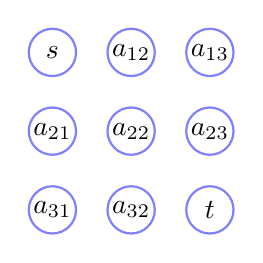
\begin{tikzpicture}
    [mine/.style={circle, draw=red!50,fill=red!70,thick,inner sep=0pt,minimum size=6mm},
    empty/.style={circle, draw=blue!50,thick,inner sep=0pt,minimum size=6mm}]
    \node[empty] (a11) at (0,0) {$s$};
    \node[empty] (a12) at (1,0) {$a_{12}$};
    \node[empty] (a13) at (2,0) {$a_{13}$};
    \node[empty] (a21) at (0,-1) {$a_{21}$};
    \node[empty] (a22) at (1,-1) {$a_{22}$};
    \node[empty] (a23) at (2,-1) {$a_{23}$};
    \node[empty] (a31) at (0,-2) {$a_{31}$};
    \node[empty] (a32) at (1,-2) {$a_{32}$};
    \node[empty] (a33) at (2,-2) {$t$};
\end{tikzpicture}
\caption{Original matrix with numbers.}
\end{minipage}%
\begin{minipage}[b]{.5\textwidth}
  \centering
  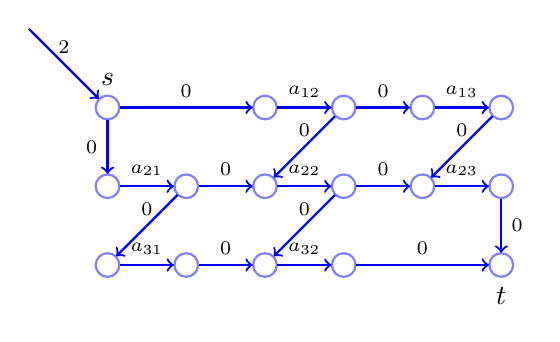
\begin{tikzpicture}
    [st/.style={circle, draw=blue!50,thick,inner sep=0pt,minimum size=6mm,scale=0.8},
    empty/.style={circle, draw=blue!50,thick,inner sep=0pt,minimum size=6mm,scale=0.5}]
    \node[empty,label=above:{$s$}] (a11) at (0,0) {};
    \node[empty] (a121) at (2,0) {};
    \node[empty] (a122) at (3,0) {};
    \node[empty] (a131) at (4,0) {};
    \node[empty] (a132) at (5,0) {};
    \node[empty] (a211) at (0,-1) {};
    \node[empty] (a212) at (1,-1) {};
    \node[empty] (a221) at (2,-1) {};
    \node[empty] (a222) at (3,-1) {};
    \node[empty] (a231) at (4,-1) {};
    \node[empty] (a232) at (5,-1) {};
    \node[empty] (a311) at (0,-2) {};
    \node[empty] (a312) at (1,-2) {};
    \node[empty] (a321) at (2,-2) {};
    \node[empty] (a322) at (3,-2) {};
    \node[empty,label=below:{$t$}] (a33) at (5,-2) {};

    \draw [->,blue,thick] (a11) -- (a121) node[above,font=\scriptsize,color=black,align=center,midway]{0};
    \draw [->,blue,thick] (a11) -- (a211) node[left,font=\scriptsize,color=black,align=center,midway]{0};
    \draw [->,blue,thick] (a121) -- (a122) node[above,font=\scriptsize,color=black,align=center,midway]{$a_{12}$};
    \draw [->,blue,thick] (a211) -- (a212) node[above,font=\scriptsize,color=black,align=center,midway]{$a_{21}$};
    \draw [->,blue,thick] (a122) -- (a131) node[above,font=\scriptsize,color=black,align=center,midway]{0};
    \draw [->,blue,thick] (a122) -- (a221) node[above,font=\scriptsize,color=black,align=center,midway]{0};
    \draw [->,blue,thick] (a131) -- (a132) node[above,font=\scriptsize,color=black,align=center,midway]{$a_{13}$};
    \draw [->,blue,thick] (a132) -- (a231) node[above,font=\scriptsize,color=black,align=center,midway]{0};
    \draw [->,blue,thick] (a212) -- (a221) node[above,font=\scriptsize,color=black,align=center,midway]{0};
    \draw [->,blue,thick] (a212) -- (a311) node[above,font=\scriptsize,color=black,align=center,midway]{0};
    \draw [->,blue,thick] (a221) -- (a222) node[above,font=\scriptsize,color=black,align=center,midway]{$a_{22}$};
    \draw [->,blue,thick] (a311) -- (a312) node[above,font=\scriptsize,color=black,align=center,midway]{$a_{31}$};
    \draw [->,blue,thick] (a222) -- (a231) node[above,font=\scriptsize,color=black,align=center,midway]{0};
    \draw [->,blue,thick] (a222) -- (a321) node[above,font=\scriptsize,color=black,align=center,midway]{0};
    \draw [->,blue,thick] (a231) -- (a232) node[above,font=\scriptsize,color=black,align=center,midway]{$a_{23}$};
    \draw [->,blue,thick] (a312) -- (a321) node[above,font=\scriptsize,color=black,align=center,midway]{0};
    \draw [->,blue,thick] (a232) -- (a33) node[right,font=\scriptsize,color=black,align=center,midway]{0};
    \draw [->,blue,thick] (a321) -- (a322) node[above,font=\scriptsize,color=black,align=center,midway]{$a_{32}$};
    \draw [->,blue,thick] (a322) -- (a33) node[above,font=\scriptsize,color=black,align=center,midway]{0};

    \draw [->,blue,thick] (-1,1) -- (a11) node[above,font=\scriptsize,color=black,align=center,midway]{2};
\end{tikzpicture}
\caption{Extended network for Figure 1,$C(e)=1$ for all edges and the weight shows on the line, the objective is 2.}
\end{minipage}
\end{figure}

We set the capacity of all edges as 1, which forces each point can't be walk through more than once. We set the cost between sub-points of one original point as the original number. One path $(s\rightarrow t\rightarrow s)$ without duplicate points equals to two paths $(s\rightarrow t),(s\rightarrow t)$ without duplicate points, so we set the objective of the extended network as 2.

By running minimum cost flow algorithm, we can find the minimal cost from $s$ to $t$ and back to $s$.

\section*{6\quad Maximum Cohesiveness}

Here is the solution excerpted from iitd\footnote{\url{http://www.cse.iitd.ac.in/~rjaiswal/2011/csl356/Notes/Week-11/lec-2.pdf}}.

Given a graph $G=<V,E,W>$, we construct a network graph $G'$ as follows.
\begin{itemize}
  \item There is a vertex $v$ corresponding to every vertex $v$ in $G$.
  \item There is a vertex $v_{ij}$ corresponding to each edge $e_{ij}$ in $G$.
  \item There is a source $s$ and a sink vertex $t$.
  \item Vertex $v_{ij}$ has edges to vertex $i$ and $j$. This has capacity $\infty$.
  \item There is an edge from $s$ to all vertexes $v_{ij}$. These edges have capacity $w_{ij}$.
  \item There is an edge from every vertex $v$ to $t$ with capacity $\alpha$.
\end{itemize}

\begin{figure}[!ht]
\centering
\begin{minipage}[b]{.5\textwidth}
  \centering
  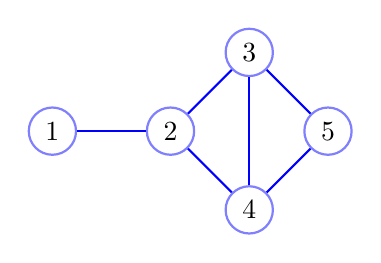
\begin{tikzpicture}
    [mine/.style={circle, draw=red!50,fill=red!70,thick,inner sep=0pt,minimum size=6mm},
    empty/.style={circle, draw=blue!50,thick,inner sep=0pt,minimum size=6mm}]
    \node[empty] (v1) at (-0.5,0) {1};
    \node[empty] (v2) at (1,0) {2};
    \node[empty] (v3) at (2,1) {3};
    \node[empty] (v4) at (2,-1) {4};
    \node[empty] (v5) at (3,0) {5};

    \draw [blue,thick] (v1) -- (v2);
    \draw [blue,thick] (v3) -- (v2);
    \draw [blue,thick] (v4) -- (v2);
    \draw [blue,thick] (v4) -- (v3);
    \draw [blue,thick] (v5) -- (v4);
    \draw [blue,thick] (v5) -- (v3);
\end{tikzpicture}
\caption{Original undirected graph $G$.}
\end{minipage}%
\begin{minipage}[b]{.5\textwidth}
  \centering
  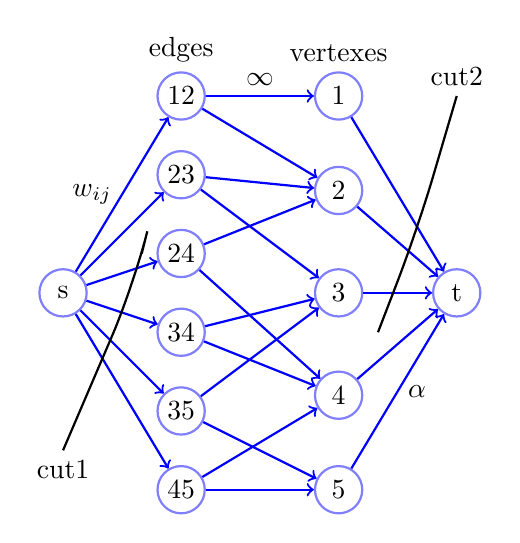
\begin{tikzpicture}
        [mine/.style={circle, draw=red!50,fill=red!70,thick,inner sep=0pt,minimum size=6mm},
        empty/.style={circle, draw=blue!50,thick,inner sep=0pt,minimum size=6mm}]
        \node[empty] (s) at (0,0) {s};
        \node[empty] (v24) at (1.5,0.5) {24};
        \node[empty] (v23) at (1.5,1.5) {23};
        \node[empty,label=above:{edges}] (v12) at (1.5,2.5) {12};
        \node[empty] (v34) at (1.5,-0.5) {34};
        \node[empty] (v35) at (1.5,-1.5) {35};
        \node[empty] (v45) at (1.5,-2.5) {45};
        \node[empty,label=above:{vertexes}] (v1) at (3.5,2.5) {1};
        \node[empty] (v2) at (3.5,1.3) {2};
        \node[empty] (v3) at (3.5,0) {3};
        \node[empty] (v4) at (3.5,-1.3) {4};
        \node[empty] (v5) at (3.5,-2.5) {5};
        \node[empty] (t) at (5,0) {t};

        \draw [->,blue,thick] (v1) -- (t);
        \draw [->,blue,thick] (v2) -- (t);
        \draw [->,blue,thick] (v3) -- (t);
        \draw [->,blue,thick] (v4) -- (t);
        \draw [->,blue,thick] (v5) -- (t) node[right,color=black,align=center,midway]{$\alpha$};

        \draw [->,blue,thick] (v12) -- (v1) node[above,color=black,align=center,midway]{$\infty$};
        \draw [->,blue,thick] (v12) -- (v2);
        \draw [->,blue,thick] (v23) -- (v2);
        \draw [->,blue,thick] (v23) -- (v3);
        \draw [->,blue,thick] (v24) -- (v2);
        \draw [->,blue,thick] (v24) -- (v4);
        \draw [->,blue,thick] (v34) -- (v4);
        \draw [->,blue,thick] (v34) -- (v3);
        \draw [->,blue,thick] (v35) -- (v5);
        \draw [->,blue,thick] (v35) -- (v3);
        \draw [->,blue,thick] (v45) -- (v4);
        \draw [->,blue,thick] (v45) -- (v5);

        \draw [<-,blue,thick] (v12) -- (s) node[left,color=black,align=center,midway]{$w_{ij}$};
        \draw [<-,blue,thick] (v23) -- (s);
        \draw [<-,blue,thick] (v34) -- (s);
        \draw [<-,blue,thick] (v24) -- (s);
        \draw [<-,blue,thick] (v35) -- (s);
        \draw [<-,blue,thick] (v45) -- (s);
        \draw [black,thick,rounded corners=20pt]  (0,-2) node[below]{cut1} -- (0.9,0.1) -- (1,0.5);
        \draw [black,thick,rounded corners=20pt] (4,-0.5) -- (4.5,0.8) -- (5,2.5) node[above]{cut2};
\end{tikzpicture}
\caption{Extended network $G'$.}
\end{minipage}
\end{figure}

Let $(A,B)$ be a min-cut in $G'$. Let $S$ be the vertexes on the right that are in $B$.

\begin{itemize}
  \item Claim 1: If $v_{ij}$ is in $A$, then both $i$ and $j$ are in $A$, otherwise $(v_{ij},i)$ or $(v_{ij},j)$ can be augmented, it isn't a maximal flow.
  \item Claim 2: If $i$ and $j$ is in $A$, then $v_{ij}$ is in $A$.
  \item Claim 3: The capacity of min cut, $C(A,B)=e(Total)-e(S)+|S|\alpha$
  \item Claim 4: There is a subset $S$ with cohesiveness $\geq \alpha$ \textbf{if and only if $C(A,B)\leq e(Total)$}.
\end{itemize}

If Claim 4 holds, we have $C(A,B)\leq e(Total)$ $\Leftrightarrow$ $e(Total)-e(S)+|S|\alpha\leq e(Total)$ $\Leftrightarrow$ $e(S)/|S|\geq\alpha$ $\Leftrightarrow$ $S$ is the maximum cohesiveness.

\rule{\textwidth}{1pt}

助教解法:

因为 $e(Total)=e(S)+e(\bar S)+e(S\bar S)$, 如果 $C(A,B)=e(\bar S)+e(S\bar S)+|S|\alpha$, 那么有

\[
\begin{array}{rrcll}
& C(A,B)& \leq & e(Total) \\
\Rightarrow & e(\bar S)+e(S\bar S)+|S|\alpha & \leq & e(S)+e(\bar S)+e(S\bar S)\\
\Rightarrow & \alpha & \leq & e(S)/|S|
\end{array} \nonumber
\]
所以$S$ 是maximum cohesiveness。下面我们来证明$C(A,B)=e(\bar S)+e(S\bar S)+|S|\alpha$。

假设最小割如Figure 4中的cut1和cut2,则$S=\{1,2,3\}$。\textcolor[rgb]{1.00,0.00,0.00}{注意割不一定要是连续的一条线,只要把$s$和$t$割开,使得$s$和$t$无法到达即可。}

\begin{enumerate}
  \item $e(S)\notin C(A,B)$. 因为$S$被割,对应残余图中边$<S,t>$已经满流,所以左边不能再流过去了,即$e(S)\notin C(A,B)$。比如Figure 4 右边割了$S=\{1,2,3\}$,则不能再割$S$内部的边,如$<1,2>$和$<2,3>$,即边$<s,12>$和$<s,23>$不会被割。
  \item $e(S\bar S)\in C(A,B)$. 如果不割$e(S\bar S)$,则边还没满流,还可以增加流量,即没有达到最大流,和当前是最小割矛盾。比如$3\in S$ 且$4\notin S$,如果边$<3,4>$即$<s,34>$没有被割,则还可以通过$s\rightarrow 34\rightarrow 4\rightarrow t$增加流量,不满足最大流,$C(A,B)$也就不是最小割了,矛盾。所以$e(S\bar S)\in C(A,B)$。
  \item $e(\bar S)\in C(A,B)$. 和2的证明类似,因为$4\notin S,5\notin S$,如果边$<s,45>$不被割,则不是最大流,所以边$<s,45>$被割,即$e(\bar S)\in C(A,B)$。
\end{enumerate}

由此得证$C(A,B)=e(\bar S)+e(S\bar S)+|S|\alpha$,进而得到$\alpha\leq e(S)/|S|$,$S$为maximum cohesiveness。
\end{document}
